% !TEX encoding = UTF-8 Unicode
% !TEX root = SystemTemplate.tex

\documentclass{book}

% !TEX root = SystemTemplate.tex

\usepackage[width=6.5in, height=9.2in, top=1.0in, papersize={8.5in,11in}]{geometry}
\usepackage[pdftex]{graphicx}
\usepackage{amsmath}
\usepackage{amsthm}
\usepackage{amssymb}
%\usepackage{txfonts}
\usepackage{textcomp}
\usepackage{amsthm}

\usepackage[all]{xy}
\usepackage{fancyhdr}
\pagestyle{fancy}
\usepackage{hyperref}
\usepackage{verbatim}
\usepackage{algorithm}
\usepackage{algorithmic}
\usepackage{array}
\usepackage{color}
\usepackage{listings}
\usepackage{calc}
\usepackage{doxygen}
\usepackage[utf8]{inputenc}
\usepackage{makeidx}
\usepackage{multicol}
\usepackage{multirow}
\usepackage[table]{xcolor}
\usepackage{tabularx}
\usepackage{framed}
\usepackage{xspace}
\usepackage{etex}
\usepackage{todonotes}
\usepackage[final]{pdfpages}
\usepackage{pgfgantt}


%% Computer Modern Bright Font
%\usepackage{cmbright}
%\usepackage[T1]{fontenc}

%% Sans Serif Modern Font - similar to  Helvetica
\usepackage{lmodern}
\renewcommand*\familydefault{\sfdefault} %% Only if the base font of the document is to be sans serif
\usepackage[T1]{fontenc}


\definecolor{SDColor1}{rgb}{0,0,0}
\definecolor{SDColor2}{rgb}{0,0,0}
\definecolor{SDColor3}{rgb}{0,0,0}
\definecolor{SDColor4}{rgb}{0,0,0}
\definecolor{SDColor5}{rgb}{0,0,0}

%%%  --- Here are some other colors.  Keep it conservative --- %%%

%% Blue font color scheme
%\definecolor{SDColor1}{rgb}{.204,.353,.541}
%\definecolor{SDColor2}{rgb}{.31,.506,.741}
%\definecolor{SDColor3}{rgb}{0.18,0.35,0.59}
%\definecolor{SDColor4}{rgb}{0.44,0.59,0.82}
%\definecolor{SDColor5}{rgb}{0.35,0.35,0.35}
%

%% Brown color scheme
% \definecolor{SDColor1}{rgb}{.55,.2,.2}
%\definecolor{SDColor2}{rgb}{.4,.1,.1}
%\definecolor{SDColor3}{rgb}{.5, .15,.15}
%\definecolor{SDColor4}{rgb}{.63,.32,.18}
%\definecolor{SDColor5}{rgb}{.45,.15,.15}
%


%% Custom colors for code listing environment
\definecolor{OliveGreen}{cmyk}{0.64,0,0.95,0.40}
\definecolor{DarkBlue}{cmyk}{0.76,0.76,0,0.20}
\definecolor{DarkRed}{cmyk}{0,1,1,0.45}
\lstset{language=c,frame=ltrb,framesep=5pt,basicstyle=\normalsize,
 keywordstyle=\ttfamily\color{DarkRed},
identifierstyle=\ttfamily\color{DarkBlue}\bfseries,
commentstyle=\color{OliveGreen},
stringstyle=\ttfamily,
showstringspaces=false,tabsize = 3}


\setlength{\oddsidemargin}{0mm} 
\setlength{\evensidemargin}{0mm} 

%% Uncomment if you want "Draft" placed on each page.
%\usepackage{draftwatermark}
%\SetWatermarkLightness{0.975}
%\SetWatermarkScale{1}
%\SetWatermarkText{Draft}

\pagestyle{fancy}
\renewcommand{\chaptermark}[1]{\markboth{#1}{}}
\renewcommand{\sectionmark}[1]{\markright{\thesection\ #1}}
\fancyhf{}
\fancyhead[LE,RO]{\bfseries\thepage}
\fancyhead[LO]{\bfseries\rightmark}
\fancyhead[RE]{\bfseries\leftmark}
%\fancyfoot[LE,RO]{Confidential and Proprietary}
%\renewcommand{\headrulewidth}{0.5pt}
%\renewcommand{\footrulewidth}{0pt}
%\addtolength{\headheight}{0.5pt}
%\setlength{\footskip}{0mm}
%\renewcommand{\footruleskip}{0pt}



\usepackage{titlesec}
\titleformat{\chapter}[display]
{\normalfont\bfseries\color{SDColor3}}    %\normalfont\bfseries\filcenter}
{\LARGE\thechapter}
{1ex}
{\titlerule[2pt]
\vspace{2ex}%
\LARGE}
[\vspace{1ex}%
{\titlerule[2pt]}]

%
%\usepackage{titlesec}
%\titleformat{\chapter}{\normalfont\bfseries\LARGE}
%{\thechapter.}{5pt}{}[{\titlerule[3pt]}]
%
%\titleformat{\section}{\normalfont\bfseries\Large}
%{\thesection.}{5pt}{}[{\titlerule[2pt]}]
%
%\titleformat{\subsection}{\normalfont\bfseries\large}
%{\thesubsection.}{5pt}{}[{\titlerule[1pt]}]
%


%\titleformat*{\section}{\Large\bfseries\sffamily\color{SDColor1}}
%\titleformat*{\subsection}{\large\bfseries\sffamily\color{MSLightBlue}}
%\titleformat*{\section}{\Large\bfseries\color{SDColor3}}
%\titleformat*{\subsection}{\large\bfseries\color{SDColor4}}

%\titleformat*{\section}{\Large\bfseries}
%\titleformat*{\subsection}{\large\bfseries}
%\titleformat*{\subsubsection}{\large\bfseries}

\titleformat*{\section}{\Large\bfseries\color{SDColor1}}  
\titleformat*{\subsection}{\large\bfseries\color{SDColor2}}
\titleformat*{\subsubsection}{\large\bfseries\color{SDColor5}}
\setcounter{secnumdepth}{3}
\renewcommand{\thesubsubsection}{\thesubsection.\alph{subsubsection}}

% Save the original chapter command as stdchapter
\let\stdchapter\chapter

%redefine the backmatter command
\let\stdbackmatter\backmatter
\makeatletter% We need the '@' letter to call if@openright
\renewcommand{\backmatter}{
\stdbackmatter
% need to set the page counter back to 1
\setcounter{page}{1}
%% Redefine the \chapter command for our Back Matter
\renewcommand{\chapter}[1]{
  \if@openright\cleardoublepage\else\clearpage\fi% chapters begin on right page
  \stdchapter{##1}% output standard chapter heading
  \setcounter{section}{0}% restart the section numbering
  \renewcommand{\thepage}{BM-\arabic{page}}% Redefine page numbering format
  \renewcommand{\thesection}{\arabic{section}}% Redefine section number format
}}
\makeatother% Restore the normal behavior of '@'

%redefine the appendix command
\let\stdappendix\appendix
\makeatletter% We need the '@' letter to call if@openright
\renewcommand{\appendix}{
\stdappendix
%% \titleformat{\chapter}[display]
%% {\normalfont\bfseries\color{SDColor3}}    %\normalfont\bfseries\filcenter}
%% {\LARGE Appendix \thechapter}
%% {1ex}
%% {\titlerule[2pt]
%% \vspace{2ex}%
%% \LARGE}
%% [\vspace{1ex}%
%% {\titlerule[2pt]}]
  %%% Since counters are different in the appendix section
  %%% we redefine \chapter to explicitly reset the page number
  %%%  (comment out to see effect)
  \renewcommand{\chapter}[1]{
    \stdchapter{##1}\setcounter{page}{1}
    %%% We also redefine page numbering
    \renewcommand{\thepage}{\Alph{chapter}-\arabic{page}}
  }
}
\makeatother% Restore the normal behavior of '@'


\makeatletter% We need the '@' letter to call if@openright
\newcommand{\agreement}{
  \renewcommand{\chapter}[1]{
    \if@openright\cleardoublepage\else\clearpage\fi% chapters begin on right page
    \pagestyle{plain}% turn off fancy headers
    \setcounter{section}{0}% Reset the section number
    \setcounter{page}{1}% Reset the page number
    \renewcommand{\thepage}{SA-\arabic{page}}% Set format for page numbering
    \renewcommand{\thesection}{\arabic{section}}% Set format for section numbering
    \refstepcounter{chapter}% Add it to the index/toc for on-line viewing
    \addcontentsline{toc}{chapter}{##1}% Add to the table of contents
  }
}
\makeatother% Restore the normal behavior of '@'



%%  If you do some math typesetting, you may want more environment names.
%% Uncomment to see how this works:
%\newtheorem{summary}{Summary:}
%\newtheorem{example}{Example:}



 % This sets the format.

% Add your title page contents here 
\title{{\color{MSBlue1} \rule{\linewidth}{0.5mm}}\\[2mm] {\huge \bfseries \color{MSBlue1} Product/Report Title Here }\\[-1mm] {\color{MSBlue1}\rule{\linewidth}{0.5mm}} \\  \vfill
{\LARGE \bfseries \color{MSBlue2} Senior Design Final Documentation }\\  \vfill 
{\color{MSBlue1} Team Name} }
\author{\color{MSBlue1}  FullName1 \and \color{MSBlue1} FullName2 \and  \color{MSBlue1} FullName3 }
\date{\color{MSBlue1} \today}


\begin{document}

\frontmatter

\addcontentsline{toc}{chapter}{Title}
\maketitle
\tableofcontents
\addcontentsline{toc}{chapter}{Contents}
\listoffigures
\addcontentsline{toc}{chapter}{List of Figures}
\listoftables
\addcontentsline{toc}{chapter}{List of Tables}
\listofalgorithms
\addcontentsline{toc}{chapter}{List of Algorithms}

\chapter{Overview Statements}
% !TEX root = DesignDocument.tex

\section{Mission Statement}
The purpose of this project is to develop a virtual reality environment that accurately represents the Ruth Brennan art exhibit at the Dahl Arts Center.  The end product will be able to be transported to and from the museum too allow students and others, who otherwise cannot visit the museum, to experience the Dahl.

\section{Elevator Pitch}
The Dahl Arts Center would like to have the ability to bring their art galleries outside the museum to the community.  In order to do this, a virtual reality gallery will be constructed to assess the viability of using this method as a means of taking the art out of the museum.  % add mission statement to mission.tex

\chapter{Document Preparation and Updates}
% !TEX root = SystemTemplate.tex



Current Version [X.X.X]
\vspace*{5mm}

{\color{MSBlue3}
\noindent
\textit{Prepared By:}\\
\textit{Team Member \#1}\\
\textit{Team Member \#2}\\
\textit{Team Member \#3}
}

\vfill
\noindent
{\color{color02} \textit{\textbf{Revision History}}}\\
\begin{tabular}{|>{\raggedright}p{1.5cm}|>{\raggedright}p{3cm}|>{\raggedright}p{1.5cm}|>{\raggedright}p{9cm}|}
\hline
\textit{\textbf{Date}} &  \textit{\textbf{Author}} & \textit{\textbf{Version}} & \textit{\textbf{Comments}}\tabularnewline
\hline
 \textit{\textbf{2/2/12}} & \textit{Team Member \#1} & \textit{1.0.0} & \textit{Initial version}\tabularnewline
\hline
\textit{\textbf{3/4/12}} & \textit{Team Member \#3} & \textit{1.1.0} & \textit{Edited version}\tabularnewline
\hline
 &  &  & \tabularnewline
 \hline
 &  &  & \tabularnewline
\hline
 &  &  & \tabularnewline
\hline
 &  &  & \tabularnewline
\hline
 &  &  & \tabularnewline
\hline
\end{tabular}
\vfill


 
\mainmatter

%%  Add to the following chapters

% !TEX root = DesignDocument.tex


\chapter{Overview and concept of operations}

The purpose of this project is to develop a virtual reality environment that accurately represents the Ruth Brennan art exhibit at the Dahl Arts Center.  The end product will be able to be transported to and from the museum too allow students and others, who otherwise cannot visit the museum, to experience the Dahl.

The end goal for this particular project is to have the prototype gallery running using the Oculus Rift and Unreal Engine.  This is so the Dahl Arts Center can get an accurate grasp of how this sort of technology will work and will inform their decision about whether to go further with the Oculus or not.  This leads to another goal for the project team, research additional methods to utilize the virtual reality of the Oculus and give the Dahl a better understanding of what is feasible and what is fantasy.

The system that is going to be used for this project uses the Unreal Engine for the environment and the Oculus Rift for the virtual reality immersion.  In order to allow users to experience this virtual gallery, there will have to be an operator who will know how to setup the Oculus and Unreal Engine for the tour to run efficiently.  

\section{Team Members and Team Name}
The team for this project, Virtual Dahl Art Gallary, consists of Alex Nienhueser and Mackenzie Smith. 

% !TEX root = SystemTemplate.tex


\section{Resumes}

%Your resumes are included here.  See the source file (industrial.tex) and uncomment the PDF includes to see how this works.  If your resume is written in \LaTeX\ then you can just insert the \LaTeX\ source code.

    \includepdf[pages={1}]{report.pdf}  %% example of limited page include

	  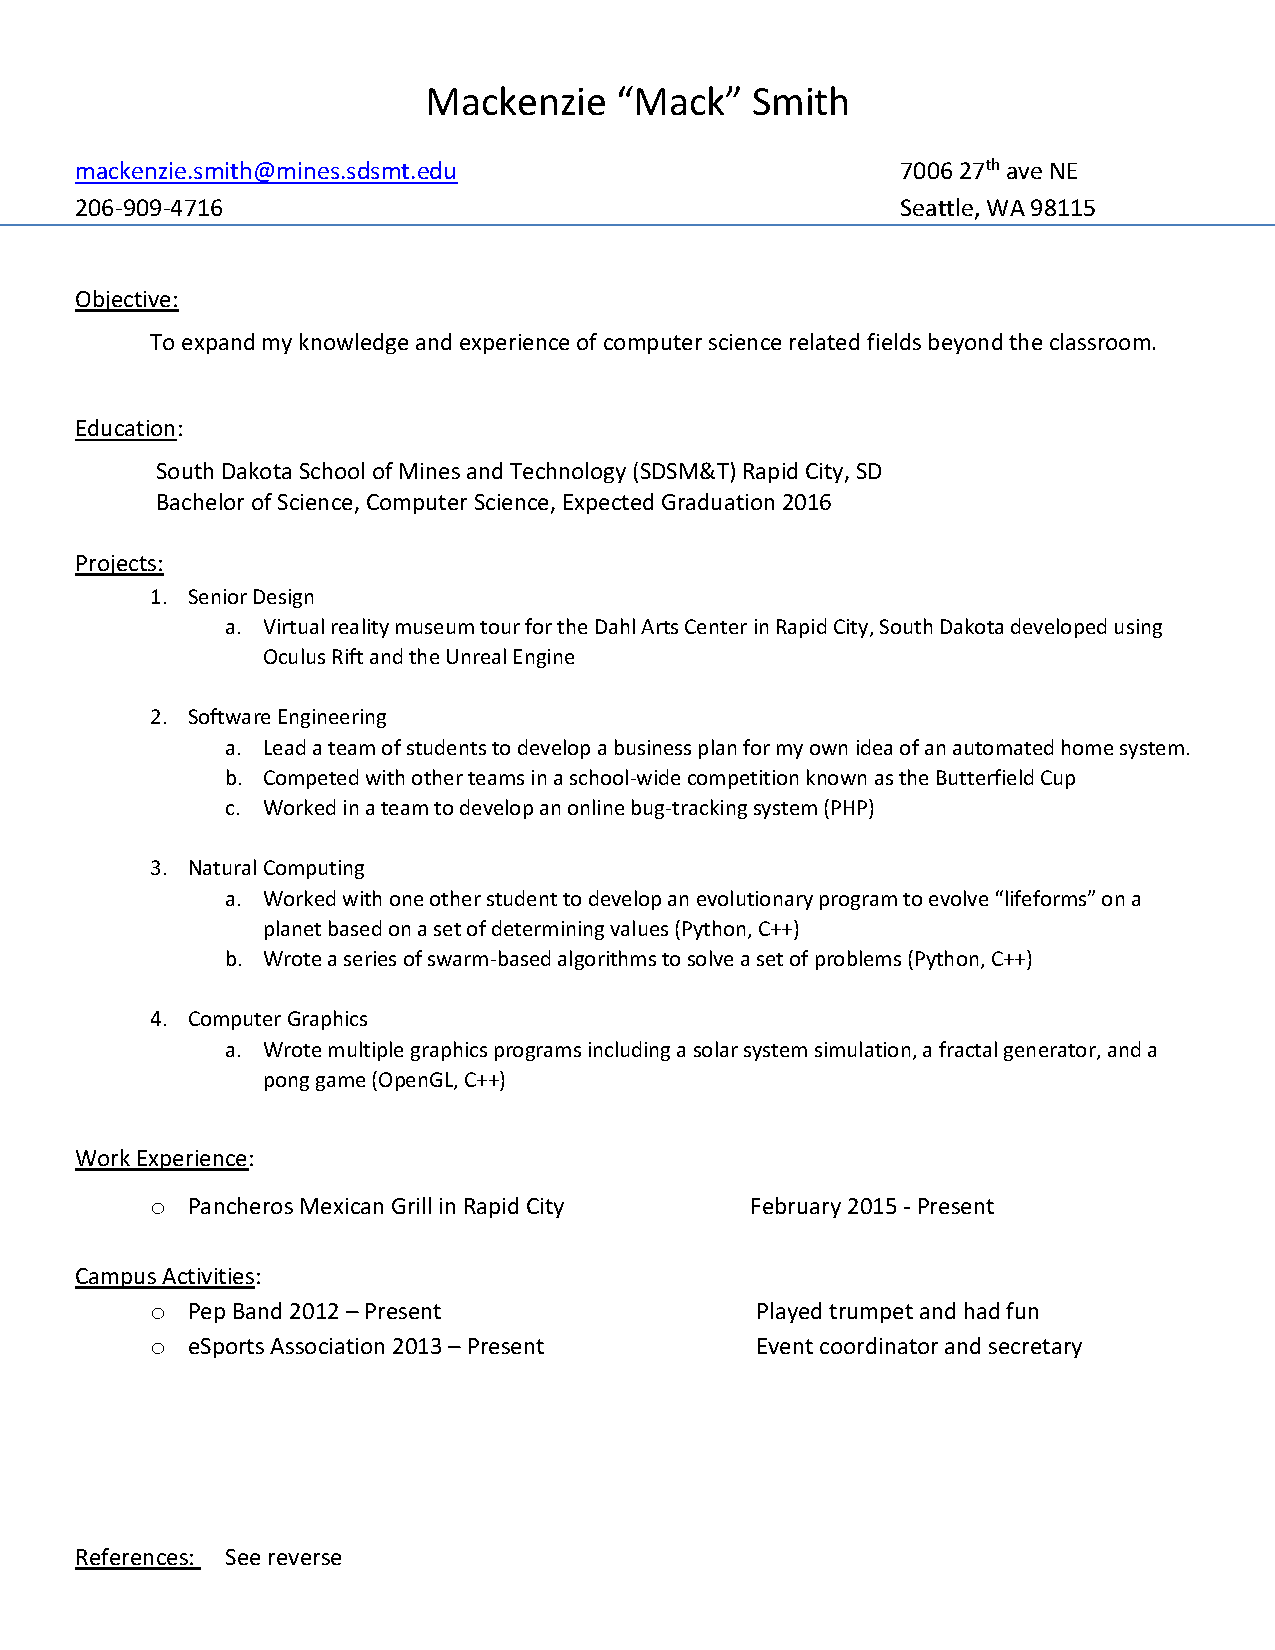
\includepdf{Resumes/Mack'sResume.pdf}
      
\includepdf{Resumes/Alex'sResume.pdf}
%     \includepdf{resume3.pdf}

\section{ABET:  Industrial Experience Reports}

\subsection{Mackenzie Smith}

% \includepdf{name1.pdf}

\subsection{Alex Nienhueser}

% \includepdf{name2.pdf}






\section{Client}
The Dahl Arts Center, located in downtown Rapid City South Dakota, is a huge supporter of local artists in and around the Black Hills area. 

\section{Project}
The Dahl Arts Center requests a virtual reality environment that is an accurate reflection of a current gallery in the museum.  This virtual gallery will allow a single user to experience the art pieces in a virtual environment via a virtual reality headset, in the case of this project the Oculus Rift.  Once the user has put the goggles on they will be able to choose between two movement options, free movement and on-rails which are explained further in the document.  After the movement method has been chosen, the user will explore the gallery at their discretion.  At a few selected paintings, text descriptions will be available that will pop up next to the corresponding painting allowing the user to read an interpretive description written by the artist.  There will also be some video recordings depicting the artist's methods.  Finally, the user will able to change the environment itself from the gallery to another scene to be determined. 

\subsection{Purpose of the System}
The purpose of the virtual gallery is give options people who are unable to travel to the Dahl Arts Center. By creating a virtual reality environment of one of the galleries it allows for users to enjoy the Dahl from their own home. 


\section{Business Need}
%Use this section to define what business need exist and how this software will 
%meet and/or exceed that business need.  
A museum is generally a place you physically travel to in order to experience it.  In order to experience the museum, you'll need to either walk or drive there which isn't possible for a large amount of people.  They might be disabled, lack the funds for transportation, or any other reason that prevents them from visiting the museum.  That's where this project will come in; by making the museum a piece of software, it will be easily transportable, apart from the hardware required to run it.  This will allow the Dahl to effectively take the museum out to those who might not be able to experience it otherwise.

\section{Deliverables}

The deliverables for this project will include:
\begin{description}
\item[Unreal Blueprints] \hfill \\
	These constitute the "code" for the project, which handles all of the user movement and animations in the gallery.  These will be needed if the Dahl decides to continue the project any further.

\item[Unreal Assets] \hfill \\
	The Unreal assets are the "physical" objects in the gallery.  These include the walls, paintings, alternate environment, etc...  These will be delivered as texture files, object files, and other file formats required for the Unreal Engine.
	
\item[User Documentation] \hfill \\
	This document will detail how to install, and operate the software developed during this project, as well as how to install and operate the Oculus Rift.

\item[Standalone Executable] \hfill \\
	This will be the project itself that will be able to be ran as a program on any computer that has the requisite software installed; e.g. the Oculus Rift drivers.
\end{description}   

\section{System Description}

\subsection{Unreal Engine 4.0}
This was the main development environment used during the development of the project.  It encompassed the peripheral integration as well as the visual scripting software (Blueprints).

\subsection{Oculus Rift}
The Oculus Rift SDK2 was the virtual reality headset that was used for implementing the VR in the Unreal Engine.  This component includes the headset as well as the software drivers necessary to run it.

\subsection{Xbox Controller}
This component is simply a wired Xbox 360 controller that was used to control user movement. 

\section{System Overview and Diagram}
Provide a more detailed description of the major system components
without getting too detailed.  This section should contain a
high-level block and/or flow diagram of the system highlighting the
major components.  See Figure~\ref{systemdiagram}.  This is a floating
figure environment.  \LaTeX\ will try to put it close to where it was
typeset but will not allow the figure to be split if moving it can not
happen.  Figures, tables, algorithms and many other floating
environments are automatically numbered and placed in the appropriate
type of table of contents.  You can move these and the numbers will
update correctly.

\begin{figure}[tbh]
\begin{center}
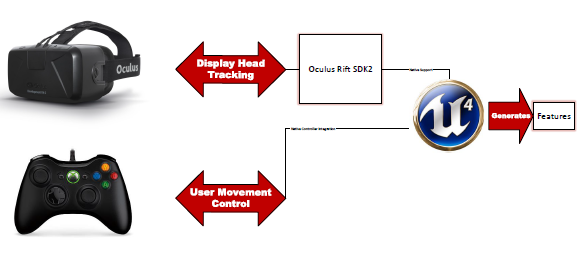
\includegraphics[width=0.75\textwidth]{Diagrams/SystemDiagram.png}
\end{center}
\caption{The overall system diagram. \label{systemdiagram}}
\end{figure}

\section{Technologies Overview}
\begin{description}
\item[Unreal Engine] \hfill \\
	The Unreal Engine was the main development environment for this project.  It had all of the facilities for integrating the movement controls, Oculus Rift, as well as the Blueprint IDE.  This technology was used to create the entire project aside from the actual paintings.  Epic Games' documentation for the Unreal Engine is very extensive and can be found here: \href{https://docs.unrealengine.com/latest/INT/}{Unreal Engine Documentation}
	
\item[Oculus Rift] \hfill \\
	The Oculus Rift was the headset used for the virtual reality implementation.  It has separate software and drivers that need to be installed before it could be used in conjunction with the Unreal Engine.  Once the drivers were installed, it can integrate seamlessly with the Engine.  Documentation on the Oculus can be found here:\href{https://developer.oculus.com/documentation/intro-vr/latest/concepts/bp_app_imaging/}{Oculus Documentation}.  Their documentation details developer best practices, which the design team implemented with the movement methods.
	
\item[Xbox Controller] \hfill \\
	The Xbox 360 controller along with any other gamepad can be integrated directly with the Unreal Engine.  This allowed the design team to simply plug the controller in and use it right away.  There is no reference material for the Xbox controller specifically, refer to Unreal Engine documentation for controller details.
\end{description}



  %% All tracks
% !TEX root = DesignDocument.tex


\chapter{Project Overview}
%This section provides some housekeeping type of information with regard to the 
%team, project, environment, etc. 



\section{Team Member's Roles}
%Describe who was involved and what role(s) were played. 
For this team Mackenzie Smith is the Project Lead. He will keep in contact with the Dahl, and interpret what they want for the project. Alex Nienhueser will be the Scrum Master. He will who's assigned specific tasks as well as their order.

\section{Project  Management Approach}
%This section will provide an explanation of the basic approach to managing the 
%project.  Typically, this would detail how the project will be managed through 
%a given Agile methodology.  The sprint length (i.e. 2 weeks) and product backlog 
%ownership and location (ex. Trello) are examples of what will be discussed.  An 
%overview of the system used to track sprint tasks, bug or trouble tickets, and 
%user stories would be warranted. 


\section{ Stakeholder Information}
This section would provide the basic description of all of the stakeholders for 
the project.  Who has an interest in the successful and/or unsuccessful completion 
of this project? 


\subsection{Customer or End User (Product Owner)}
The Product owner is the Dahl Arts Center, they will be determining the direction the project go. They will provide feedback on what features should be in this project, as well as user stories.They will be kept up to date by Mackenzie Smith on both the backlog as well as the progress of the project.
%Who?  What role will they play in the project?  Will this person or group manage 
%and prioritize the product backlog?  Who will they interact with on the team to 
%drive product backlog priorities if not done directly? 

\subsection{Management or Instructor (Scrum Master)}
The Scrum Master for this project is Alex Nienhueser. He will be determining the order in which key features are to be finished and test. He will also determine Sprint Meeting times. 
%Who?  What role will they play in the project?  Will the Scrum Master drive the 
%Sprint Meetings? 


\subsection{Investors}
For this project there are no current investors. It there is no money going to the this Virtual Gallery.
%Are there any?  Who?  What role will they play? 


\subsection{Developers --Testers}
The developers and designers for this project are both Mackenzie Smith and Alex Nienhueser, wihle the Project Manager is only Mackenzie Smith. Testing will be done via participants of beta testing times done throughout the projects development. These participants will be SDSMT students and faculty. 
%Who?  Is there a defined project manager, developer, tester, designer, architect, 
%etc.? 

\section{Budget}
For this project there is no current budget. Due to the Unreal 4 Engine's libary of textures there is no need to purchase any additional enviorment. 

\section{Intellectual Property and Licensing}
This will be looked further into in sprint 4.
%Describe the IP ownership and issues surrounding IP.

\section{Sprint  Overview}
If the system will be implemented in phases, describe those phases/sub-phases (design, 
implementation, testing, delivery) and the various milestones in this section. 
 This section should also contain a correlation between the phases of development 
and the associated versioning of the system, i.e. major version, minor version, 
revision. 

All of the Agile decisions are listed here.  For example, how do you order your backlog?   
Did you use planning poker?   

\section{Terminology and Acronyms}
Provide a list of terms used in the document that warrant definition.  Consider 
industry or domain specific terms and acronyms as well as system specific. 

\section{Sprint Schedule}
See Table 3.1
\begin{table}[]
\centering
\caption{My caption}
\label{my-label}
\begin{tabular}{lllllll}
                                                                                              &                                                                                                                                             &                                                                                                                        &                                                                                                                       &                                                                                         &                                          &                                                                                          \\ \hline
\multicolumn{1}{|l|}{\begin{tabular}[c]{@{}l@{}}Sprint 1 Start\\ Date 9/14/15\end{tabular}}   & \multicolumn{1}{l|}{\begin{tabular}[c]{@{}l@{}}Research Oculus \\ and Limitations 9/23/15\end{tabular}}                                     & \multicolumn{1}{l|}{\begin{tabular}[c]{@{}l@{}}Familiarize with \\ Unreal Engine 10/1/15\end{tabular}}                 & \multicolumn{1}{l|}{\begin{tabular}[c]{@{}l@{}}End of Sprint 1\\ 10/2/15\end{tabular}}                                & \multicolumn{1}{l|}{}                                                                   & \multicolumn{1}{l|}{}                    & \multicolumn{1}{l|}{}                                                                    \\ \hline
\multicolumn{1}{|l|}{\begin{tabular}[c]{@{}l@{}}Sprint 2 Start \\ Date 10/12/15\end{tabular}} & \multicolumn{1}{l|}{\begin{tabular}[c]{@{}l@{}}Create Draft of \\ Gallery in Unreal\\ 10/17/15\end{tabular}}                                & \multicolumn{1}{l|}{\begin{tabular}[c]{@{}l@{}}Begin Prototype of \\ Free Movement\\ 10/20/15\end{tabular}}            & \multicolumn{1}{l|}{\begin{tabular}[c]{@{}l@{}}Begin Prototype of On \\ Rails Movement \\ 10/24/15\end{tabular}}      & \multicolumn{1}{l|}{\begin{tabular}[c]{@{}l@{}}End of Sprint 2\\ 10/30/15\end{tabular}} & \multicolumn{1}{l|}{}                    & \multicolumn{1}{l|}{}                                                                    \\ \hline
\multicolumn{1}{|l|}{\begin{tabular}[c]{@{}l@{}}Sprint 3 Start \\ Date 11/9/15\end{tabular}}  & \multicolumn{1}{l|}{\begin{tabular}[c]{@{}l@{}}Finish Free Movement \\ 11/17/15\end{tabular}}                                               & \multicolumn{1}{l|}{\begin{tabular}[c]{@{}l@{}}Finish On Rails Movement\\ 11/25/15\end{tabular}}                       & \multicolumn{1}{l|}{Finalize Gallery Inviornment 11/26/15}                                                            & \multicolumn{1}{l|}{\begin{tabular}[c]{@{}l@{}}End of Sprint 3\\ 10/30/15\end{tabular}} & \multicolumn{1}{l|}{}                    & \multicolumn{1}{l|}{}                                                                    \\ \hline
\multicolumn{1}{|l|}{\begin{tabular}[c]{@{}l@{}}Sprint 4 Start\\ Date 1/18/15\end{tabular}}   & \multicolumn{1}{l|}{\begin{tabular}[c]{@{}l@{}}Create Prototype of Ray Tracing\\ 1/21/15\end{tabular}}                                      & \multicolumn{1}{l|}{\begin{tabular}[c]{@{}l@{}}Test Ray Tracing on \\ Painting Description\\ 1/26/15\end{tabular}}     & \multicolumn{1}{l|}{\begin{tabular}[c]{@{}l@{}}Apply and Test Ray \\ Tracing to All Paintings\\ 1/30/15\end{tabular}} & \multicolumn{1}{l|}{End of Sprint 4 2/5/16}                                             & \multicolumn{1}{l|}{}                    & \multicolumn{1}{l|}{}                                                                    \\ \hline
\multicolumn{1}{|l|}{\begin{tabular}[c]{@{}l@{}}Sprint 5 Start \\ Date 2/15/16\end{tabular}}  & \multicolumn{1}{l|}{\begin{tabular}[c]{@{}l@{}}Determine Basic Design \\ and Structure of Alternate \\ Environment.\\ 2/21/16\end{tabular}} & \multicolumn{1}{l|}{\begin{tabular}[c]{@{}l@{}}Create Rough Draft \\ of Alternate Environment.\\ 2/29/16\end{tabular}} & \multicolumn{1}{l|}{\begin{tabular}[c]{@{}l@{}}Finalize Alt. Environment\\ 3/2/16\end{tabular}}                       & \multicolumn{1}{l|}{\begin{tabular}[c]{@{}l@{}}End of Sprint 5\\ 3/4/16\end{tabular}}   & \multicolumn{1}{l|}{}                    & \multicolumn{1}{l|}{}                                                                    \\ \hline
\multicolumn{1}{|l|}{Sprint 5 Start Date 3/21/16}                                             & \multicolumn{1}{l|}{\begin{tabular}[c]{@{}l@{}}Finish any Remaining \\ Work from Previous Sprints\end{tabular}}                             & \multicolumn{1}{l|}{\begin{tabular}[c]{@{}l@{}}Finish all Testing \\ on all Movement.\end{tabular}}                    & \multicolumn{1}{l|}{Implement User Friendly}                                                                          & \multicolumn{1}{l|}{Finish Documentation}                                               & \multicolumn{1}{l|}{Finish Deleverables} & \multicolumn{1}{l|}{\begin{tabular}[c]{@{}l@{}}End of Sprint 6 \\ 4/15/16,\end{tabular}} \\ \hline
\end{tabular}
\end{table}

\section{Timeline}
Gantt chart or other type of visual representation of the project timeline.

\section{Backlogs}
%Place the sprint backlogs here.    The product backlog will be in the chapter with the user 
%stories.

\section{Burndown Charts}
Place your burndown charts, team velocity information, etc here.   


\section{Development Environment}
The development environment for this project is the Unreal 4 Engine. To run this project it will need to be loaded into the Unreal 4 Engine ver 9.2. If version 9.2 can't be downloaded then Unreal 4 has tool to convert the project to any newer version of the software.
%The basic purpose for this section is to give a developer all of the necessary 
%information to setup their development environment to run, test, and/or develop. 


\section{Development IDE and Tools}
The two IDE's used for this project are the Unreal 4 Engine and Visual Studios
%Describe which IDE and provide links to installs and/or reference material. 

\section{Source  Control}
The source control used for this project is GitHub. We had it set up with four current directories. The first being blueprints. This contains all of the blueprints for the Unreal Engine as well as any other code we create or generate. The next directory is Documentation\_new. This contains the newest DesignDocument as well as the project contract. There is a similar directory Documentation\_old which contains the an older version of  Documentation\_new. Finally the last directory, SprintReports, contains report for each sprint for this project.
%Which source control system is/was used?  How was it setup?  How does a developer 
%connect to it? 

\section{Dependencies}
Describe all dependencies associated with developing the system. 

\section{Build  Environment}
The build environment for this project is all handled by the Unreal 4 Engine.
%How are the packages built?  Are there build scripts? 

\section{Development Machine Setup}
For setup the user will need an Oculus Rift. Once it is unpackaged the user will need to plug the hdmi cord from the Oculus headset to their computers graphics card. 
%If warranted, provide a list of steps and details associated with setting up a 
%machine for use by a developer. 


   %% All tracks
% !TEX root = DesignDocument.tex

\chapter{User Stories,  Requirements, and Product Backlog}
\section{Overview}

The Dahl Arts Center in Rapid City has asked for some way to be able to bring their art from the galleries to the community.  Dr. King Adkins, who brought this project to the school, thought of the idea of using virtual reality to recreate a gallery without risking any of the actual pieces.  Through meetings with the Dahl Arts Committee, user stories were developed which made the project feasible within the course of the senior design class.

The Dahl listed a total of four user stories which were then reworked in order to read the requirements from them.  The original as well as the reworked user stories will be included in the user story section of this document to show that no details were lost when reworking them.  

There will be a number of design constraints and system requirement as well, such as a minimum level of hardware to run the Unreal Engine; this will be discussed in the requirements section.  

Finally, the product backlog will be spelled out showing all of the pieces of the product that need to be produced in the course of this project. 






\section{User Stories}
%This section can really be seen as the guts of the document.  This section should 
%be the result of discussions with the stakeholders with regard to the actual functional 
%requirements of the software.  It is the user stories that will be used in the 
%work breakdown structure to build tasks to fill the product backlog for implementation 
%through the sprints.
%
%This section should contain sub-sections to define and potentially provide a breakdown 
%of larger user stories into smaller user stories.   Each component must have a test identified, 
%meaning you need to know how you plan to test it.  If a requirement is not testable, then 
%some justification needs to be made on why the requirement has been included.  
% The results of the tests should go in the testing chapter. 

The user stories given by the Dahl Arts Center seemed to focus more on what they wanted to get out of this product rather than how the user should be using it.  That being said, the senior design team developed more constrained user stories directly from those provided by the Dahl.  Both versions will be included in this document to ensure that no features were left out of the reworked user stories.  In some cases, pieces of different user stories were taken to produce a more relevant user story.



\subsection{User Story \#1 Original}
Create a virtual and interactive gallery space that mimics the space of one of our galleries, preferably the Ruth Brennan Gallery. 

\subsection{User Story \#1 Revised}
As a user I will be able to view and interact with a virtual gallery, preferably Ruth Brennan, in a room generated using the Unreal Engine as per the room layout provided by the Dahl.

\subsubsection{User Story \#1 Breakdown}
This user story requires that the senior design team create a scale replica of an existing room in the Dahl Arts Center, the Ruth Brennan Gallery.  This will be done using the Unreal Engine by using measurements both taken in the gallery by the team, as well as a blueprint of the room provided by the Dahl.  

Testing will focus on finding glitches in the room itself such as:  holes in textures, collision detection errors (clipping through walls), and lighting

\hrulefill

\subsection{User Story \#2 Original} 
Users would be able to "step" into the gallery by placing the virtual reality goggles on and move around using a handheld controller. This technology will allow us to go out into the community and make our galleries and artwork accessible to all. 

\subsection{User Story \#2 Revised}
As a user I will be able to select between a guided tour and user-controlled experience the latter will be controlled using a handheld game controller.

\subsubsection{User Story \#2 Breakdown}
The revised user story takes some aspects from user stories 2 and 3, due to the fact that 3 had many unrelated aspects of the product.  The main topic of this user story is movement through the virtual gallery.  One method will be entirely user controlled with a handheld game controller, for this project the design team will be using an Xbox 360 Wired controller.  The other method has been termed "On-rails" meaning that the user will move between set points in the gallery along a fixed path (rails) and will not be able to freely explore the gallery.

Testing for On-rails movement will be done using unit tests for on rails in particular in ensure that when the user presses the next button, they go to the next painting in order.  These tests will be done for each painting in the gallery.

As for the free movement, the senior design team will be asking volunteers to experience the gallery and give feedback as to how nauseous the movement made them feel.  Other questions will be about if the movement was too fast or too slow which will also be included in the On-rails movement.  

\hrulefill

\subsection{User Story \#3 Original} 
The user should be able to move through the virtual space, either on a specific track or on their own path, and walk up to each work of art to view it and to view interpretive text. We also would like to see the opportunity to embed a video as one component of the exhibit. Another component we would like to have is audio interpretation. 

\subsection{User Story \#3 Revised}
As a user I will be able to view an art piece and have a description text box appear on the side of the piece with interpretive text about the piece in view.  There should also be the ability to add a short video to play on specific exhibits to add further description for the user.

\subsubsection{User Story \#3 Breakdown}
The first sentence of the original user story was included in user story 2 leaving the rest in its own user story.  The purpose of this user story is to allow the user to read an interpretive description, written by the artist, while viewing the corresponding art piece.  The description will enlarge when viewing the piece to allow easy reading, and then shrink back down when not viewing.  Video excerpts can be used in place of text descriptions in the same manner. 

Testing will for text/video descriptions will need to test if the descriptions enlarge only when looking at a piece, and shrink only when not viewing.  The design team came up with the idea of using another actor in the Unreal Engine that will act as the user, this way the team can see when this actor looks at a painting if the description will enlarge or shrink.

\hrulefill

\subsection{User Story \#4 Original}
This virtual space should be designed with a high school aged person in mind but should be accessible to all levels of education.

\subsection{User Story \#4 Revised}
This product should be able to be transported to make it able to take to other locations and allow people who might otherwise be able to experience the Dahl.

\subsection{User Story \#4 Breakdown}
The original user story does not provide very much direction for the project and ultimately isn't something the senior design team can control.  The revised user story takes into account the fact that the Dahl wanted this product to be somewhat transportable and so that is a goal of the senior design team.  

Testing for this user story isn't very possible because testing if something is transportable is only a question of whether the transportation is adequate.  Fortunately this product will only consist of a computer capable of running the Unreal Engine, and the Oculus Rift goggles themselves.

\hrulefill

\section{Requirements and Design Constraints}
Use this section to discuss what requirements exist that deal with meeting the 
business need.  These requirements might equate to design constraints which can 
take the form of system, network, and/or user constraints.  Examples:  Windows 
Server only, iOS only, slow network constraints, or no offline, local storage capabilities. 


\subsection{System  Requirements}
There are some system requirements, mainly a graphics card that is capable of running the Unreal Engine smoothly to avoid any framerate drops that could adversely affect the user experience.  Other requirements are the Oculus Rift drivers that must be installed for the Oculus to operate.


\subsection{Network Requirements}
There are no network requirements for this project.


\subsection{Development Environment Requirements}
Since this project is begin developed in the Unreal Engine, anything short of the final product will have to be experienced on a computer with the Engine installed.  The final product will be cross-platform as long as the end computer can handle the graphics load.

\subsection{Project  Management Methodology}
No official meeting schedule was established, however the design team agreed to meet with Dr. Adkins hopefully twice a month but at least once a month to discuss progress.  Dr. Adkins said he will not require written reports and that the meetings will suffice.


\section{Specifications}
Any specifications that need to be understood?  Put it here.  

\section{Product Backlog}
%The full product backlog should go here.  The sprint backlogs are located in the project chapter.
\begin{enumerate}
	\item Gallery room, textures, and lighting
	\item Apply paintings as textures
	\item Implement the video segments in their proper places in the gallery
	\item Place each painting in the correct place in the gallery
	\item Develop free-movement and on-rails tours
	\item Text descriptions
	\item Alternate environments
	\item Final documentation, user manuals/guides
\end{enumerate}
 
\begin{itemize}
\item What system will be used to keep track of the backlogs and sprint status?
\item Will all parties have access to the Sprint and Product Backlogs?
\item How many Sprints will encompass this particular project?
\item How long are the Sprint Cycles?
\item Are there restrictions on source control? 
\end{itemize}


\section{Research or Proof of Concept Results}
This section is reserved for the discussion centered on any research that needed 
to take place before full system design.  The research efforts may have led to 
the need to actually provide a proof of concept for approval by the stakeholders. 
 The proof of concept might even go to the extent of a user interface design or 
mockups. 


\section{Supporting Material}


This document might contain references or supporting material which should be documented 
and discussed  either here if appropriate or more often in the appendices at the end.  This material may have been provided by the stakeholders  
or it may be material garnered from research tasks.

  %% Not research track

% !TEX root = DesignDocument.tex

\chapter{Design  and Implementation}
%%This section is used to describe the design details for each of the major components 
%%in the system.    Note that this chapter is critical for all tracks.  Research tracks would do experimental design here where other tracks would include the engineering design aspects.    This section is not brief and requires the necessary detail that 
%%can be used by the reader to truly understand the architecture and implementation 
%details without having to dig into the code.    Sample algorithm:  Algorithm~\ref{alg1}.  This algorithm environment is automatically placed - meaning it floats.   You don't have to worry about placement or numbering.  
The Dahl Virtual Museum project will be done entirely in the Unreal Engine 4.0 using the built in Blueprint system (a visual scripting IDE).  This system provides powerful premade code segments that can be linked together in many ways, there will be images of this system in action later in the document.  The Blueprint system may not be able to cover everything that the project requires, so to make up for that, C++ code can be directly integrated into the Engine as well.  

This section will detail the different aspects of the Blueprints that will constitute the code of this project.  There will be screenshots of the blueprints of each aspect of the project, which are: movement(free and on-rails), the room, the paintings, text descriptions, and alternate environments. 
 


%Citations look like~\cite{Choset:2005:PRM, arkin2009governing, lavalle2006}  and~\cite{wiki:asimo,lumelsky:1987, nolfi2000evolutionary}.  These are done automatically.  Just fill in the database {\tt designrefs.bib} using the same field structure as the other entries.  Then pdflatex the document, bibtex the document and pdflatex twice again.  The first pdflatex creates requests for bibliography entries.
%The bibtex extracts and formats the requested entries.  The next pdflatex puts them in order and assigns labels.  The final pdflatex replaces references in the text with the assigned labels.
%The bibliography is automatically constructed.  
 
 \section{Architecture and System Design}
 The architecture and system diagrams will one and the same, and should be fairly self-explanatory.  
 The Unreal Engine 4.0 that was used for this project is very capable and already had Oculus Rift integration, which helped focus the development on the user experience and visual quality rather than getting the hardware to work together.  Installing the Oculus Rift drivers and associated software was a large chunk of sprint 1.   
 
 %put picture of architecture and system diagrams
 %\includegraphics[scale=1.0]{•}
 
 \subsection{Design Selection}
 There were a number of ways to do this project, with other graphics engines or virtual reality headsets.  The reason the Unreal Engine was chosen was because of its almost seamless integration of the Oculus Rift SDK2.  As for the Oculus Rift, that was chosen because there was an available SDK2 from Nick Newell at Echostar who graciously lent the dev kit to the design team to use.  
 
 \subsection{Data Structures and Algorithms}
 The Unreal Engine employs a number of objects that have different attributes associated with them. This section will go over the objects used in this project and why they were chosen.
 
 % list of actors, arrays, objects etc 
  
 \subsection{Data Flow}
  
 
 \subsection{Communications}
 This section will explain how each object interacts with the others, for instance how the waypoint system for the On-rails movement works. 
 
 \subsection{Classes}
 
 %\subsection{UML}
 
 %\subsection{GUI}
 
 %\subsection{MVVM, etc}

\section{ Movement }

\subsection{Technologies  Used}
\begin{enumerate}
	\item Unreal Engine Blueprint
	\item Oculus Rift
	\item Keyboard and mouse
	\item Xbox 360 wired controller
\end{enumerate}

\subsection{Component  Overview}

% SHOULD REVISE THIS SECTION
\begin{enumerate}
	\item Free movement:  User can freely move throughout the environment
	\item On-rails:  User travels from painting to painting along a linear path
\end{enumerate}

%\subsection{Phase Overview}
%This is an extension of the Phase Overview above, but specific to this component. 
% It is meant to be basically a brief list with space for marking the phase status. 

\subsection{ Architecture  Diagram}
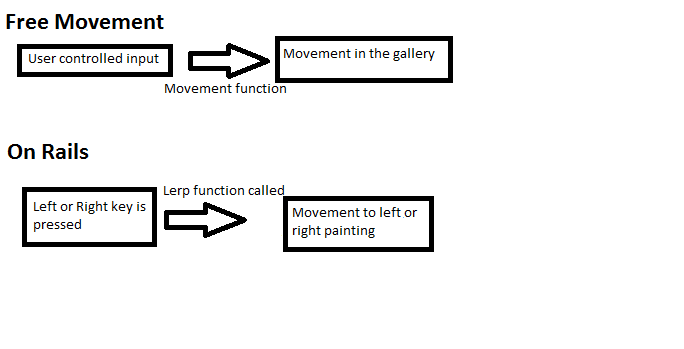
\includegraphics[scale=1.0]{Diagrams/MovementDiagram.png}


%\subsection{Data Flow Diagram}
%INSERT BLUEPRINTS HERE


\subsection{Design Details}
The movement methods are a key feature to this product.  Without a good movement system, the user will not feel immersed in the gallery and will detract from the experience.  The reason for two different methods is that the design team felt that on-rails would be a better fit for users who are inexperienced with virtual reality or handheld controller input.  The free-movement will be a better fit for people who have experience with virtual reality, or computer graphics in general.

%Should probably add more to this section



\section{Paintings }

\subsection{Technologies  Used}
\begin{enumerate}
\item Unreal Engine 4.0 Blueprint system
\end{enumerate}

\subsection{Component  Overview}
\begin{enumerate}
\item Painting image files (.png)
\item Painting texture files
\item UE objects with textures attached
\end{enumerate}

%\subsection{Phase Overview}
%I'm not exactly sure what to put for this or any of the phase overviews 

\subsection{ Architecture  Diagram}
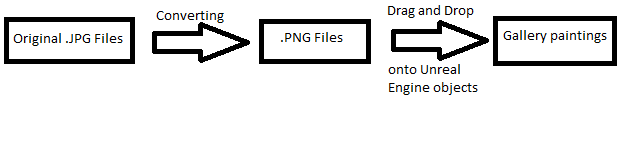
\includegraphics[scale=1.0]{Diagrams/PictureDiagram.png}
 
\subsection{Data Flow Diagram}
%INSERT BLUEPRINTS HERE


\subsection{Design Details}
This was a tedious process due to the fact that every file had to be converted from .jpg to .png in order for them to work in the engine.  Then was the task of making the objects in the right dimension for each painting which was done by making box objects to scale with the width and height of each painting, then dragging the .png file onto the object itself thereby creating the texture.


\section{Gallery }

\subsection{Technologies  Used}
\begin{enumerate}
\item Unreal Engine 4.0
\item Measuring Tape
\end{enumerate}


\subsection{Component  Overview}
The gallery itself was fairly easy to generate.  A blueprint of the actual room was provided by the Dahl and make rendering the Unreal Engine as simple as make the right sized objects.  The four outer walls were very easy to generate from the blueprint, the two protruding walls had to be measured by hand. The rounded corners however were more difficult to recreate because there are no rounded walls in the Unreal Engine, so they had to be custom made.  

%WHAT DO WE PUT FOR PHASE OVERVIEW
%\subsection{Phase Overview}
%This is an extension of the Phase Overview above, but specific to this component. 
% It is meant to be basically a brief list with space for marking the phase status. 

\subsection{ Architecture  Diagram}
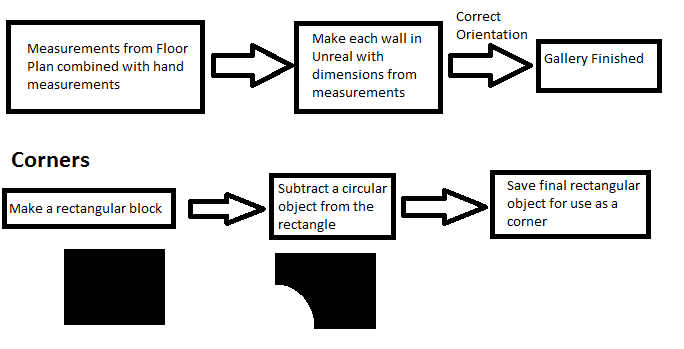
\includegraphics[scale=1.0]{Diagrams/GalleryDiagram.png}


%\subsection{Data Flow Diagram}
%INSERT BLUEPRINTS HERE



\subsection{Design Details}
This section is about how the actual room was recreated in the Unreal Engine.  The Dahl provided a blueprint of the room which gave the dimensions and angles of the corners which was helpful in mapping it into the engine.  A measuring tape was used for the standalone walls that protrude into the room and the measurements were then scaled to the Unreal Engine unit system.

\section{Text Descriptions}

\subsection{Technologies Used}
	\begin{enumerate}
		\item Unreal Engine 4.0
	\end{enumerate}

\subsection{Component Overview}
The text descriptions as described in the user stories, are interpretive excerpts written by the artist Arthur Amiotte that give insight into the meaning behind the piece.  The way the design team implemented these descriptions in the gallery is by using small rectangular objects that expand when the user is looking at the painting, in order to provide ease of reading, and then shrink back down when the user moves on.  The actual text that will appear on this object will come from a .png file and just like the paintings, be applied to in-gallery objects. 

\subsection{Architecture Diagram}
\subsection{Data Flow Diagram}
%INSERT BLUEPRINTS HERE

\subsection{Design Details}
This component was designed very similarly to the paintings, in that the method of applying this "text-texture" to the in-gallery objects was the same.  The main difference between the two, is the enlarging and shrinking of the object.  This was done using a blueprint in the Unreal Engine Blueprint editor, the blueprint itself can be viewed above in the Data Flow Diagram section.  

\section{Alternate Environment}
\subsection{Technologies Used}
\begin{enumerate}
\item terrain.party:  height map generator
\item Unreal Engine height map integrator
\end{enumerate}
\subsection{Component Overview}
\subsection{Architecture Diagram}
\subsection{Data Flow Diagram}
\subsection{Design Details}

  %% All tracks
% !TEX root = DesignDocument.tex


\chapter{System  and Unit Testing}

This section describes the approach taken with regard to system and unit testing. 

\section{Overview}
Provides a brief overview of the testing approach, testing frameworks, and general 
how testing is/will be done to provide a measure of success for the system. 

Each requirement (user story component) should be tested.    A review of objectives and
constraints might be needed here.  

\section{Dependencies}
Describe the basic dependencies which should include unit testing frameworks and 
reference material. 


\section{Test Setup and Execution}
Describe how test cases were developed, setup, and executed.  This section can 
be extremely involved if a complete list of test cases was warranted for the system.   One 
approach is to list each requirement, module, or component and describe the test.

The unit tests are described here.

\section{System Testing}

\section{System Integration Analysis}

\section{Risk Analysis}

\subsection{Risk Mitigation}

\section{Successes, Issues and Problems}

\subsection{Changes to the Backlog}

  %% All tracks
% !TEX root = SystemTemplate.tex
\chapter{Development Environment}
The basic purpose for this section is to give a developer all of the necessary 
information to setup their development environment to run, test, and/or develop. 


\section{Development IDE and Tools}
Describe which IDE and provide links to installs and/or reference material. 

\section{Source  Control}
Which source control system is/was used?  How was it setup?  How does a developer 
connect to it? 

\section{Dependencies}
Describe all dependencies associated with developing the system. 

\section{Build  Environment}
How are the packages built?  Are there build scripts? 

\section{Development Machine Setup}
If warranted, provide a list of steps and details associated with setting up a 
machine for use by a developer. 

 %% All tracks
% !TEX encoding = UTF-8 Unicode
% !TEX root = DesignDocument.tex
\chapter{Release -- Setup -- Deployment}
This section will explain the setup and initialization of the Virtual Museum. It will be seperated into details about the hardware used to run the program, how to launch the program in exe, and launching in the Unreal Engine 4's Editor (Most of this is repeated in the User Documentation).


\section{Deployment Information and Dependencies}
Are there dependencies that are not embedded into the system install? 



\section{Setup Information}

\subsection{Occulus SDK Installation}
Before you can use the SDK, you need set up the drivers for your operating system. If your drivers are already set up, please skip to the  section. This content repeats the instructions in the Oculus Rift User Guide. The first thing to do is, download the Oculus Runtime Installer from the Oculus website. The Runtime is available from https://developer.oculus.com/downloads/.
\\ This will install the following components:
\\
\\Oculus Display Driver (Windows Only)
\\ Oculus Positional Tracking Sensor Driver
\\ Oculus Service Application
\\ Oculus System Tray Application and Configuration Utility Windows
\\

\subsection{Occulus Drivers-Windows}

This section describes how to install the Windows Runtime Package.
\\
\\To install the package:
\\
\\
Download the runtime from https://developer.oculus.com/downloads/. In the Windows Control Panel, go to Programs -> Programs and Features and uninstall any existing components. Run the install executable found in this package. This will install all the components described above and prompt you to restart your computer. Restart your computer. If you want to remove the Runtime package for the current user, run the provided Uninstaller or run the OculusDirectory/Agent/uninstallAgent.sh shell script from the command line.


\subsection{Occulus Drivers-Mac}

This section describe how to install the Mac Runtime Package.
\\
\\
To install the package:
\\
\\
Download the runtime from https://developer.oculus.com/downloads/. Run the installer application found inside the package. This will install all components described above for the current user only. You must run the installer for each user that wants to use the Rift.
Since the MacOS does not currently support direct rendering, you must adjust your display settings to rotate the display by 90 degrees for the Oculus Rift DK2. The display settings are located in System Preferences -> Displays. Additionally, consider disabling display mirroring via the Mirror Displays check box on the display adjustment tab.
If you want to remove the Runtime package for the current user, run the provided Uninstaller or run the OculusDirectory/Agent/uninstallAgent.sh shell script from the command line.

\subsection{Setting Up Occulus Rift Hardware}
This section will explain how to set up the Occulus using the SDK2.
Connect your DK2 headset to your computer, following the included Instruction Manual (which can also be found online).
Run the Oculus Configuration Utility by Right-clicking on the Oculus icon in the system tray and selecting Configuration Utility. When opened, the Oculus Configuration Utility will look like the following image.\\ 
\\
\begin{center}
\centering
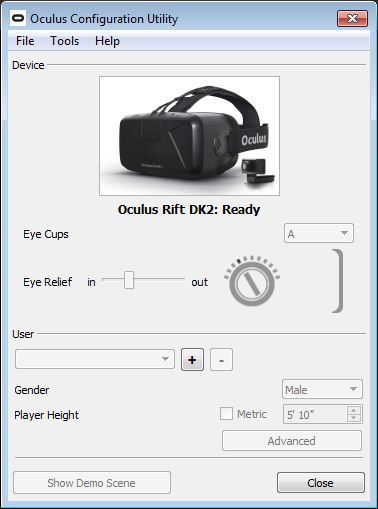
\includegraphics[scale=0.75]{Oculus_Config_Utility}\\
\end{center}
Under the User section press the Plus Sign to add a new User profile, as seen below\\
\begin{center}
\centering
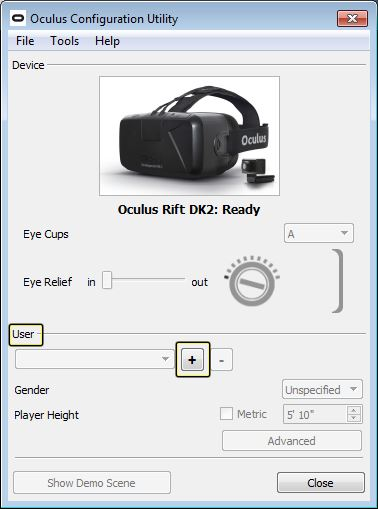
\includegraphics[scale=0.75]{Oculus_Config_Add_Profile}\\
\end{center}
In the New User pop up box that is displayed enter a name for the profile and then click the OK button.
\begin{center}
\centering
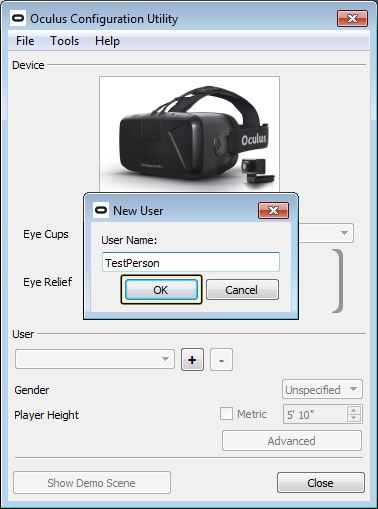
\includegraphics[scale=0.75]{Oculus_Config_Name_Profile}\\
\end{center}
Then set the in the User section set the Gender to the gender of the person using the Head Mounted Display(HMD) and set the Player Height to that persons height.
\begin{center}
\centering
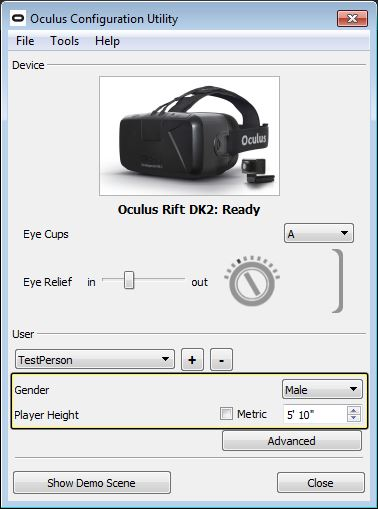
\includegraphics[scale=0.75]{Oculus_Config_Setup_Profile}\\
\end{center}
Click the Show Demo Scene button on the Oculus Configuration Utility and you should now see something similar to the following image being displayed on screen as well as being displayed in the HMD.S
\begin{center}
\centering
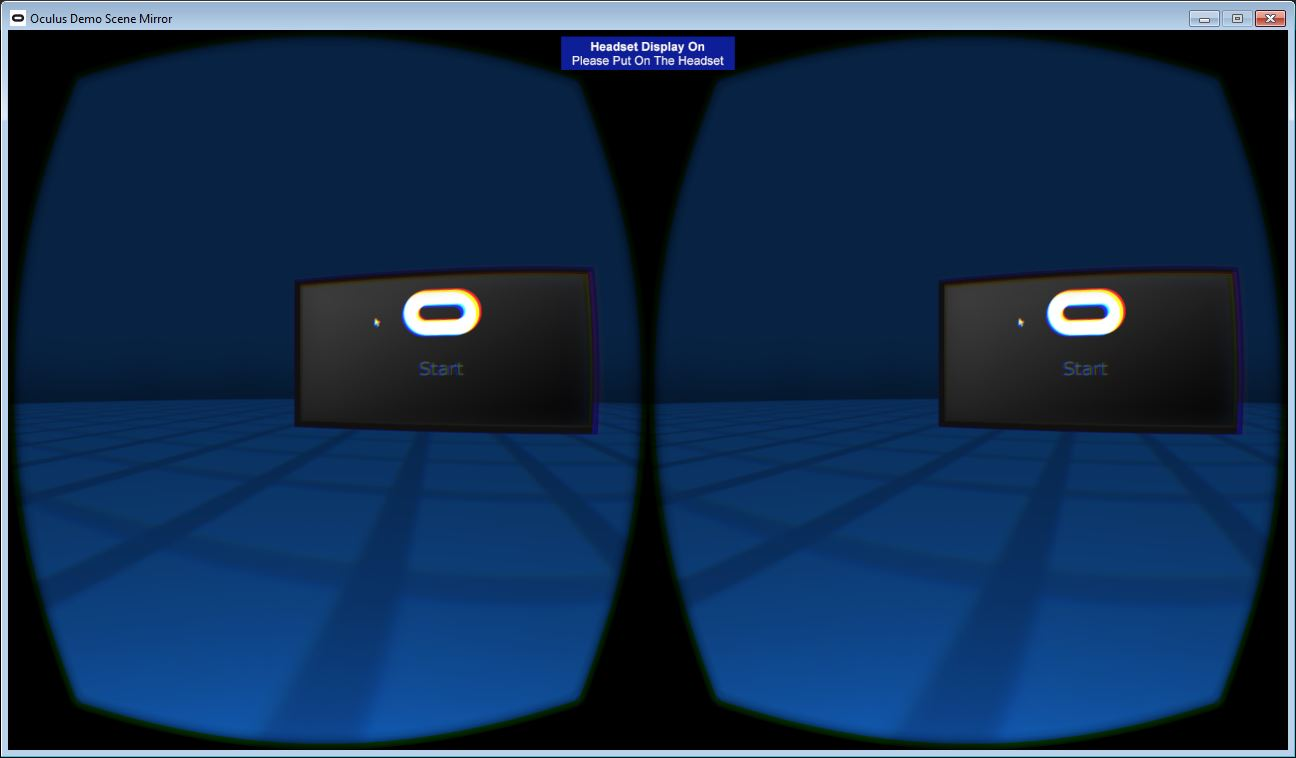
\includegraphics[scale=0.35]{Oculus_Config_Demo_Sceen}\\
\end{center}


\subsection{Unreal 4 Developement Engine}
This section will cover how to download the Unreal 4 Engine. First you will have to go to \url{https://www.unrealengine.com/what-is-unreal-engine-4} and click the get unreal button. It will then link you to  a create new user page, fill out the information and press create. The following page will then ask for a End User License Agreement. After reading it check the `I have read and agree to the End User License Agreement` check box, then click accept. It will then prompt a download button. After clicking this it will begin the downlaod for the Unreal Developement Engine.


\section{System  Versioning Information}

  %% Normally not research track
% !TEX root = SystemTemplate.tex

\chapter{User Documentation}

This section should contain the basis for any end user documentation for the system. 
 End user documentation would cover the basic steps for setup and use of the system. 
 It is likely that the majority of this section would be present in its own document 
to be delivered to the end user.  However, it is recommended the original is contained 
and maintained in this document. 

%\newpage   %% 
%%  The user guide can be an external document which is included here if necessary ...
%%  a single source is the way to go.

\section{User Guide}

The source for the user guide can go here.    You have some options for how to handle the user docs.  If you have some {\tt newpage} commands around the guide then you can just print out those pages.   If a different formatting is required, then have the source in a separate file {\tt userguide.tex} and include that file here.  That file can also be included into a driver (like the senior design template) which has the client specified formatting.  Again, this is a single source approach.   


%% \newpage  %%  if needed ...
\section{Installation Guide}


%% \newpage  %%  if needed ...
\section{Programmer Manual}

 %% All tracks
% !TEX root = SystemTemplate.tex

\chapter{Class Index}
% !TEX encoding = UTF-8 Unicode
% !TEX root = DesignDocument.tex


\section{Class List}
Here are the classes, structs, unions and interfaces with brief descriptions\-:\begin{DoxyCompactList}
\item\contentsline{section}{\hyperlink{class_poly}{Poly} }{\pageref{class_poly}}{}
\end{DoxyCompactList}

\chapter{Class Documentation}
\hypertarget{class_poly}{\section{Poly Class Reference}
\label{class_poly}\index{Poly@{Poly}}
}
\subsection*{Public Member Functions}
\begin{DoxyCompactItemize}
\item 
\hyperlink{class_poly_aa3def076b74bed67904976ad4f9fe9b1}{Poly} ()
\item 
\hyperlink{class_poly_a2f8530284140c31c0aa391dd4d0b61be}{$\sim$\-Poly} ()
\item 
int \hyperlink{class_poly_a14a7ad77ce612b0c54f531d307ee4b39}{myfunction} (int)
\end{DoxyCompactItemize}


\subsection{Constructor \& Destructor Documentation}
\hypertarget{class_poly_aa3def076b74bed67904976ad4f9fe9b1}{\index{Poly@{Poly}!Poly@{Poly}}
\index{Poly@{Poly}!Poly@{Poly}}
\subsubsection[{Poly}]{\setlength{\rightskip}{0pt plus 5cm}Poly\-::\-Poly (
\begin{DoxyParamCaption}
{}
\end{DoxyParamCaption}
)}}\label{class_poly_aa3def076b74bed67904976ad4f9fe9b1}
My constructor \hypertarget{class_poly_a2f8530284140c31c0aa391dd4d0b61be}{\index{Poly@{Poly}!$\sim$\-Poly@{$\sim$\-Poly}}
\index{$\sim$\-Poly@{$\sim$\-Poly}!Poly@{Poly}}
\subsubsection[{$\sim$\-Poly}]{\setlength{\rightskip}{0pt plus 5cm}Poly\-::$\sim$\-Poly (
\begin{DoxyParamCaption}
{}
\end{DoxyParamCaption}
)}}\label{class_poly_a2f8530284140c31c0aa391dd4d0b61be}
My destructor 

\subsection{Member Function Documentation}
\hypertarget{class_poly_a14a7ad77ce612b0c54f531d307ee4b39}{\index{Poly@{Poly}!myfunction@{myfunction}}
\index{myfunction@{myfunction}!Poly@{Poly}}
\subsubsection[{myfunction}]{\setlength{\rightskip}{0pt plus 5cm}int Poly\-::myfunction (
\begin{DoxyParamCaption}
\item[{int}]{a}
\end{DoxyParamCaption}
)}}\label{class_poly_a14a7ad77ce612b0c54f531d307ee4b39}
my own example function fancy new function

new variable 

The documentation for this class was generated from the following file\-:\begin{DoxyCompactItemize}
\item 
hello.\-cpp\end{DoxyCompactItemize}

  %% All tracks
% !TEX encoding = UTF-8 Unicode
% !TEX root = DesignDocument.tex

\chapter{Business Plan}



\section{Business Model}

\section{Market and Competition}

\section{Regulatory environment}

\section{Intellectual Property and Freedom to Operate}

\section{Management Team and Advisors}

\section{Sources and Uses of Capital}

\section{Financial Statements}

\section{Metrics and Milestones}

\section{Exit Plan}

   %% Entrepreneur track only 
% !TEX root = DesignDocument.tex


\chapter{Experimental Log}

For research projects one needs to keep a log of all research/lab activities.   

%% If you have multiple labs, you may want to break the labs into sections, check 
%% with the profession on format.
%% \section{Lab 1}

\begin{description}
\item [10/15/15]  Ran modified filter on data sets 1 - 6.  Results were ...
\item [10/17/15]  Changed tolerance on sensor and collected data.  These ...
\end{description}   %% Research track  only
% !TEX root = SystemTemplate.tex

\chapter{Research Results}

This chapter describes the results and conclusions of your research.   This would be the final report for a research project.  

\section{Result 1}

\section{Result 2}

\section{Conclusions}

\section{Further work}    %% Research track  only

\bibliographystyle{plain}
\bibliography{designrefs.bib}
\addcontentsline{toc}{chapter}{Bibliography}


% We want to add the Software agreement to the end and number the
% pages separately from the document.  We don't want to do a standard
% chapter heading, but we do want it to appear in the table of contents
% and in the index used for on-line viewing.  We defined the \agreement
% macro to set things up for us.
\agreement

\chapter{Software Agreement}
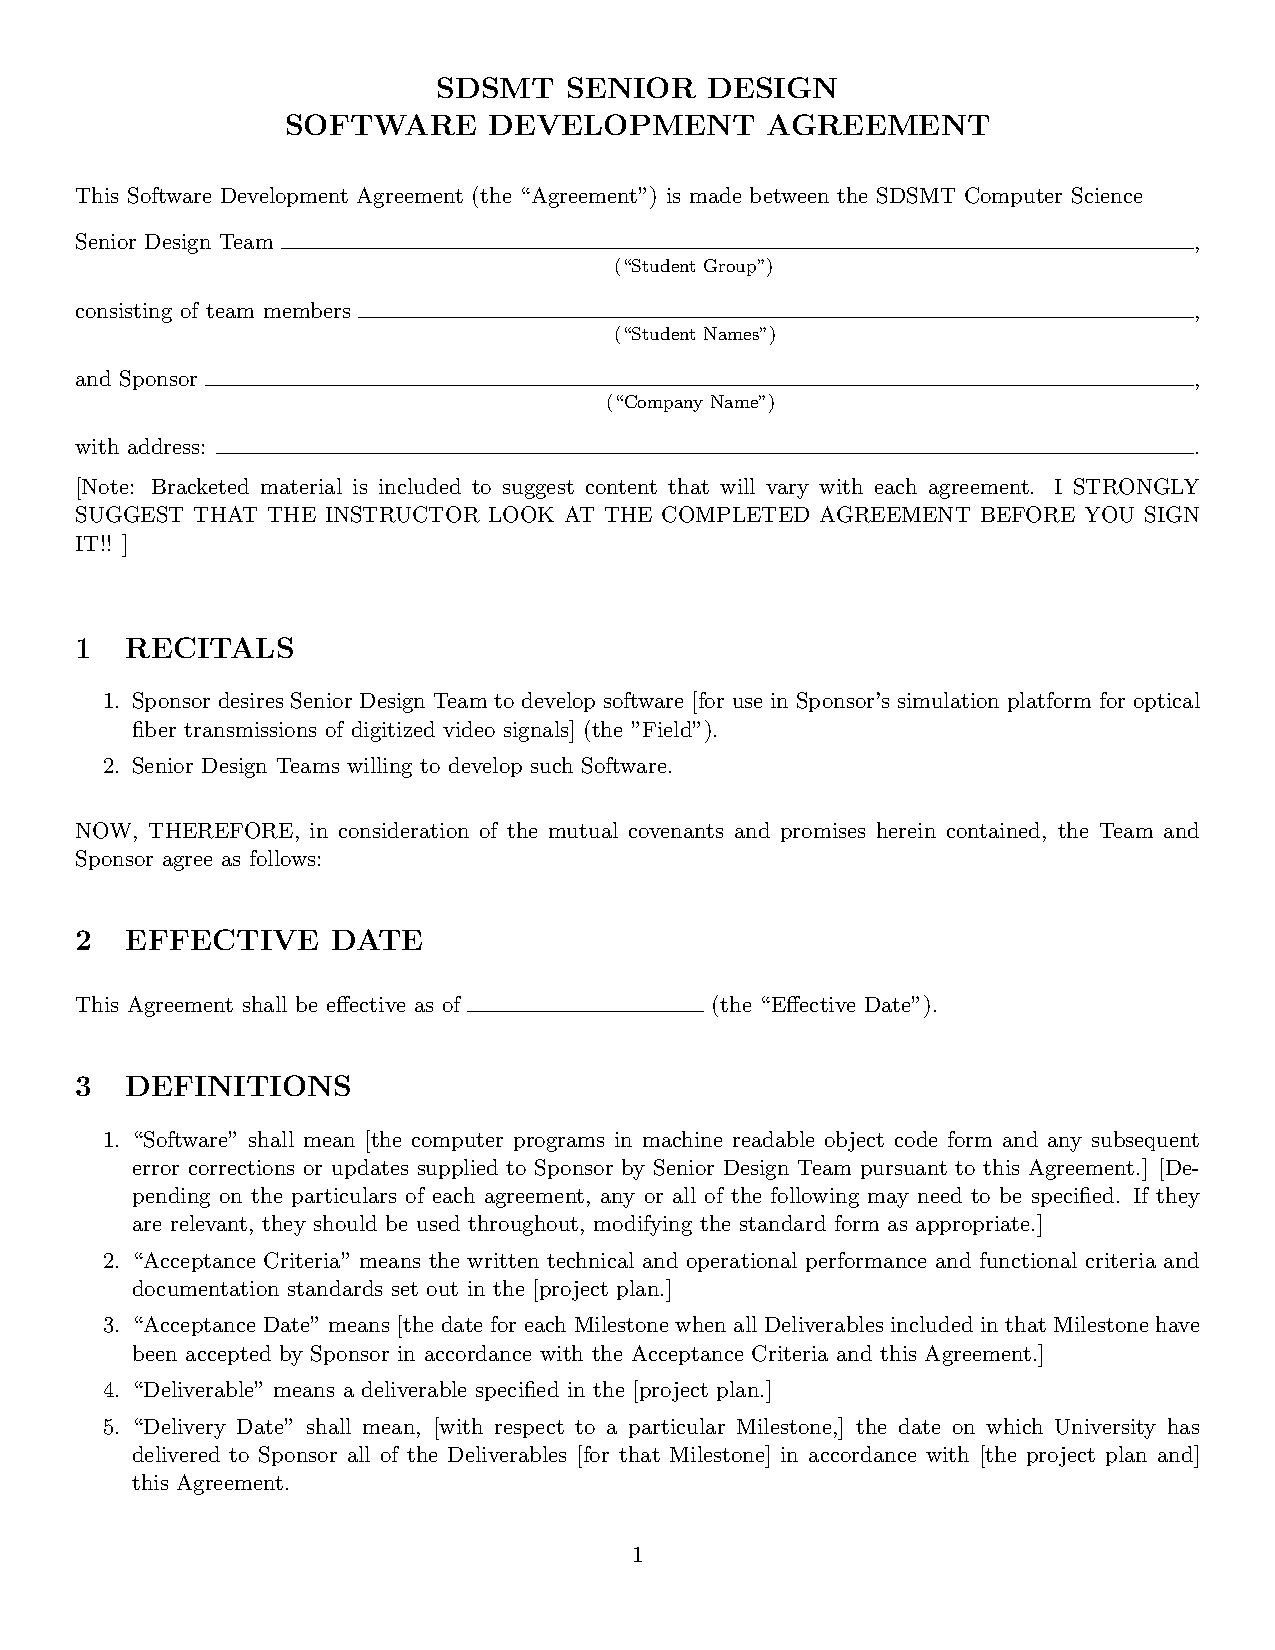
\includepdf[pages={1-5}]{SoftwareContract.pdf}

% In our style file, appendices are numbered with capital letters
\appendix

\chapter{Product Description}


The product being designed in this project will be a virtual reality museum tour of an art gallery from the Dahl Arts Center.  The gallery will be the Ruth Brennan Gallery featuring works from artist Arthur Amiotte.  The gallery will be recreated in the Unreal Engine using an Oculus Rift DK2 for virtual reality support.  

There will be two different tour choices, free movement (meaning the user can move around the gallery freely), and on-rails where the user can move between predetermined points.  Movement will be controlled by either mouse and keyboard or by using an Xbox 360 wired controller, depending on user preference.


Other features will include:
\begin{description}
\item Interpretive text descriptions \hfill \\
	These will designed to help the viewer understand the meaning behind the specific painting.  They will be written for a high school reading level, by the artist himself.  Only a few specific painting will receive these descriptions, while every painting will have a short description that are associate with every painting in the Dahl.  These short descriptions include the dimensions of the piece as well as price (if that piece is for sale).
	
\item Alternate Environment \hfill \\
	The alternate environment desired by the Dahl is the Black Hills, due to the significance between it and the author.  This will be an alternate setting in which the gallery will be recreated, to express the possibilities  of virtual reality.  
\end{description}
\vspace{2\baselineskip}

\centerline{\Large {\bf NOTE:} {\em This is part of the contract.}}



\chapter{Publications}   %% Research track 
% !TEX root = SystemTemplate.tex


Research Track:  
This chapter will include any publications generated from the research.  Most likely these will be preprints and one will just include the pdf.

%\includepdf[pages={1-5}]{Pub1.pdf}



\chapter{Sprint Reports}
% !TEX root = SystemTemplate.tex


\section{Sprint Report \#1}
The sprint reports should be inserted here.     Reports focus on process.  Design elements can be inserted into the design chapter with the report discussing the design element in more of an overview fashion.

\section{Sprint Report \#2}

\section{Sprint Report \#3}

\section{Sprint Report ...}


\chapter{Industrial Experience and Resumes}
% !TEX root = SystemTemplate.tex


\section{Resumes}

%Your resumes are included here.  See the source file (industrial.tex) and uncomment the PDF includes to see how this works.  If your resume is written in \LaTeX\ then you can just insert the \LaTeX\ source code.

    \includepdf[pages={1}]{report.pdf}  %% example of limited page include

	  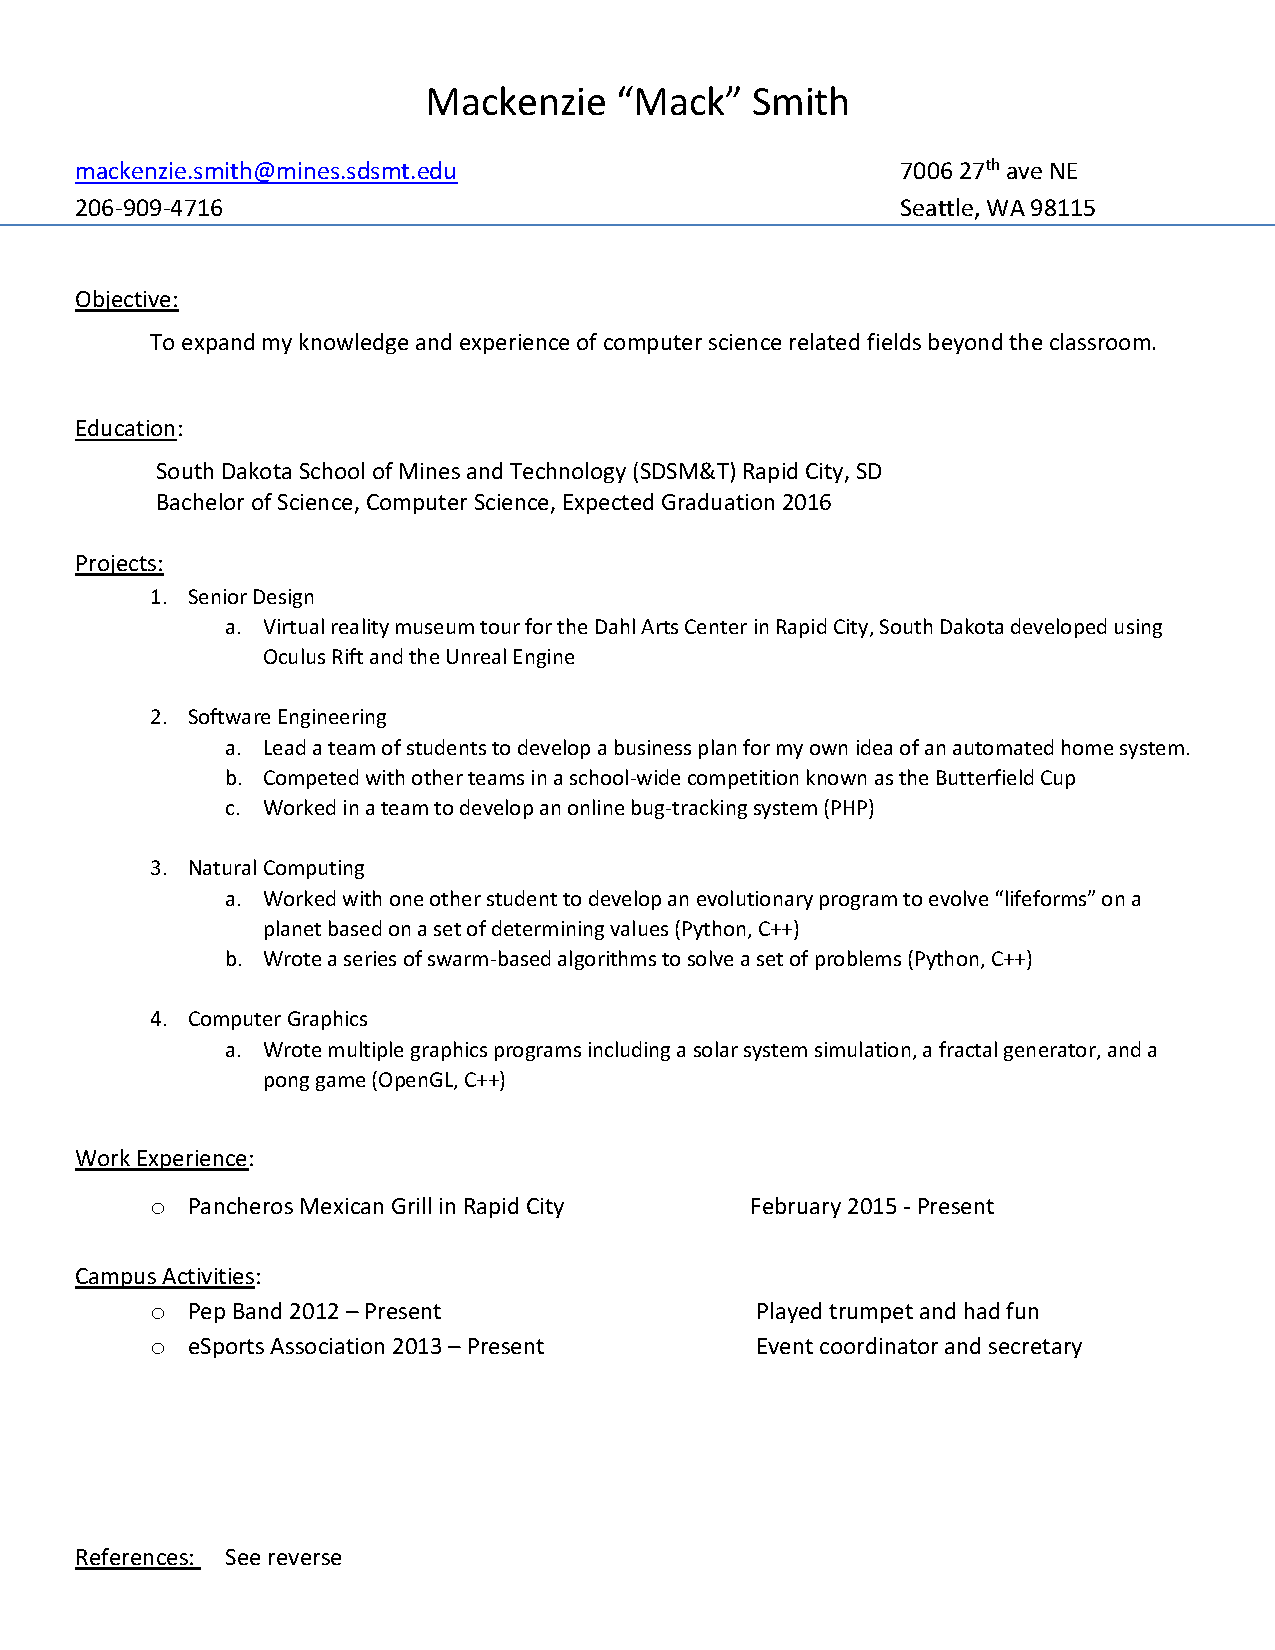
\includepdf{Resumes/Mack'sResume.pdf}
      
\includepdf{Resumes/Alex'sResume.pdf}
%     \includepdf{resume3.pdf}

\section{ABET:  Industrial Experience Reports}

\subsection{Mackenzie Smith}

% \includepdf{name1.pdf}

\subsection{Alex Nienhueser}

% \includepdf{name2.pdf}






\chapter{Acknowledgment}
\label{SpecialThanks}  
Thanks  

\chapter{Supporting Materials}

This document will contain several appendices used as a way to separate out major 
component details, logic details, or tables of information.  Use of this structure 
will help keep the document clean, readable, and organized. 



% chapters in backmatter don't have numbers, but they appear in the
% table of contents, and are numbered BM-X where X is the page number
% relative to where the backmatter begins.
\backmatter

%% Example
%\chapter{Course Syllabus}
%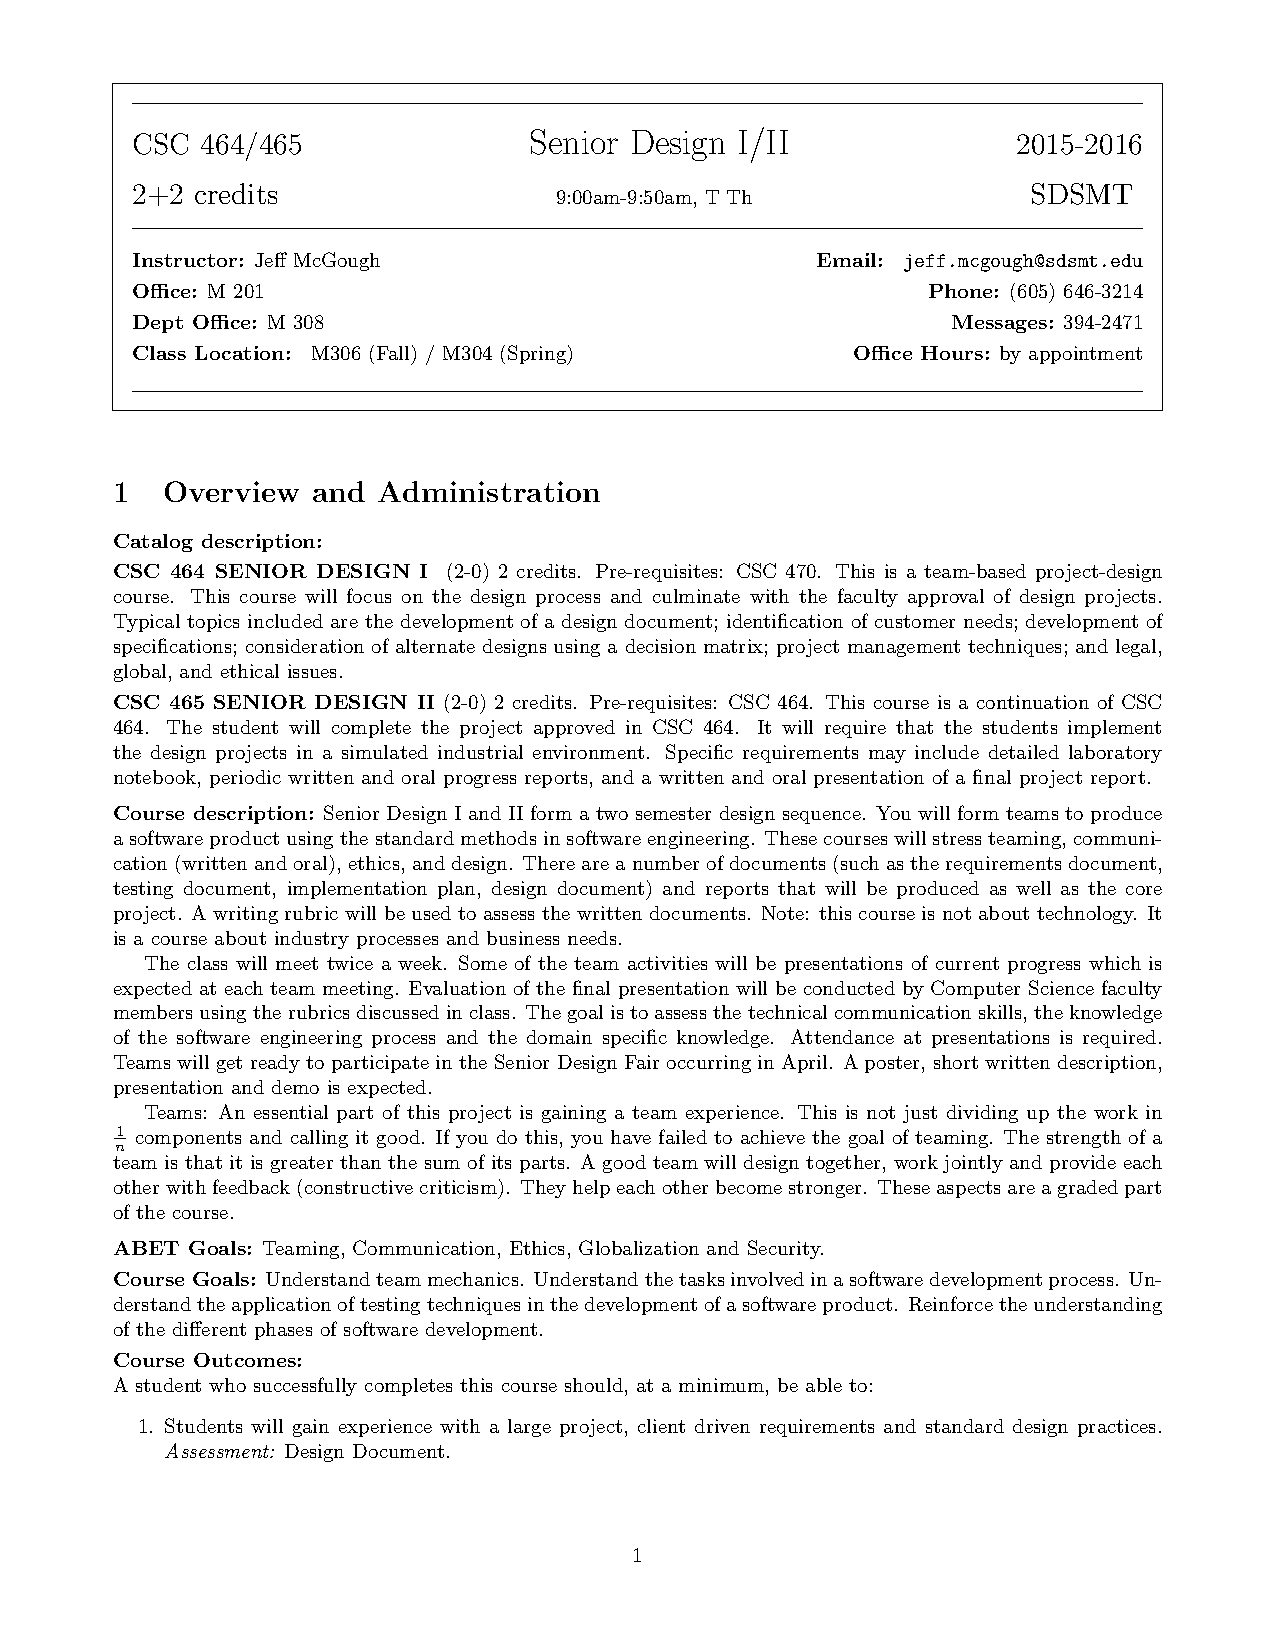
\includepdf[pages={1-17}]{syllabus.pdf}

%%% Remove after reading
\chapter{\LaTeX\ Example}
% !TEX root = DesignDocument.tex


\LaTeX\xspace sample file:  {\color{red} Remove from submitted materials}

\section{Introduction}
This is a sample input file.  Comparing it with the output it
generates can show you how to produce a simple document of
your own.

\section{Ordinary Text}  % Produces section heading.  Lower-level
                                    % sections are begun with similar 
                                    % \subsection and \subsubsection commands.

The ends  of words and sentences are marked 
  by   spaces. It  doesn't matter how many 
spaces    you type; one is as good as 100.  The
end of   a line counts as a space.

One   or more   blank lines denote the  end 
of  a paragraph.  

Since any number of consecutive spaces are treated like a single
one, the formatting of the input file makes no difference to
      \TeX,         % The \TeX command generates the TeX logo.
but it makes a difference to you.  
When you use
      \LaTeX,       % The \LaTeX command generates the LaTeX logo.
making your input file as easy to read as possible
will be a great help as you write your document and when you
change it.  This sample file shows how you can add comments to
your own input file.

Because printing is different from typewriting, there are a 
number of things that you have to do differently when preparing 
an input file than if you were just typing the document directly.  
Quotation marks like 
       ``this'' 
have to be handled specially, as do quotes within quotes: 
       ``\,`this'                  % \, separates the double and single quote.
        is what I just 
        wrote, not  `that'\,''.  

Dashes come in three sizes: an 
       intra-word 
dash, a medium dash for number ranges like 
       1--2, 
and a punctuation 
       dash---like 
this.

A sentence-ending space should be larger than the space between words
within a sentence.  You sometimes have to type special commands in
conjunction with punctuation characters to get this right, as in the
following sentence.
       Gnats, gnus, etc.\    % `\ ' makes an inter-word space.
       all begin with G\@.   % \@ marks end-of-sentence punctuation.
You should check the spaces after periods when reading your output to
make sure you haven't forgotten any special cases.
Generating an ellipsis 
       \ldots\    % `\ ' needed because TeX ignores spaces after 
                  % command names like \ldots made from \ + letters.
                  %
                  % Note how a `%' character causes TeX to ignore the 
                  % end of the input line, so these blank lines do not
                  % start a new paragraph.
with the right spacing around the periods 
requires a special  command.  

\TeX\ interprets some common characters as commands, so you must type
special commands to generate them.  These characters include the
following: 
       \$ \& \% \# \{ and \}.

In printing, text is emphasized by using an
       {\em italic\/}  % The \/ command produces the tiny extra space that
                       % should be added between a slanted and a following
                       % unslanted letter.
type style.  

\begin{em}
   A long segment of text can also be emphasized in this way.  Text within
   such a segment given additional emphasis 
          with\/ {\em Roman} 
   type.  Italic type loses its ability to emphasize and become simply
   distracting when used excessively.  
\end{em}

It is sometimes necessary to prevent \TeX\ from breaking a line where
it might otherwise do so.  This may be at a space, as between the
``Mr.'' and ``Jones'' in
       ``Mr.~Jones'',        % ~ produces an unbreakable interword space.
or within a word---especially when the word is a symbol like
       \mbox{\em itemnum\/} 
that makes little sense when hyphenated across 
       lines.

Footnotes\footnote{This is an example of a footnote.}
pose no problem.

\TeX\ is good at typesetting mathematical formulas like
       \( x-3y = 7 \) 
or
       \( a_{1} > x^{2n} / y^{2n} > x' \).
Remember that a letter like
       $x$        % $ ... $  and  \( ... \)  are equivalent
is a formula when it denotes a mathematical symbol, and should
be treated as one.

\section{Displayed Text}

Text is displayed by indenting it from the left margin.
Quotations are commonly displayed.  There are short quotations
\begin{quote}
   This is a short a quotation.  It consists of a 
   single paragraph of text.  There is no paragraph
   indentation.
\end{quote}
and longer ones.
\begin{quotation}
   This is a longer quotation.  It consists of two paragraphs
   of text.  The beginning of each paragraph is indicated
   by an extra indentation.

   This is the second paragraph of the quotation.  It is just
   as dull as the first paragraph.
\end{quotation}
Another frequently-displayed structure is a list.
The following is an example of an {\em itemized} list.
\begin{itemize}
   \item  This is the first item of an itemized list.  Each item 
          in the list is marked with a ``tick''.  The document
          style determines what kind of tick mark is used.

   \item  This is the second item of the list.  It contains another
          list nested inside it.  The inner list is an {\em enumerated}
          list.
          \begin{enumerate}
              \item This is the first item of an enumerated list that
                    is nested within the itemized list.

              \item This is the second item of the inner list.  \LaTeX\
                    allows you to nest lists deeper than you really should.
          \end{enumerate}
          This is the rest of the second item of the outer list.  It
          is no more interesting than any other part of the item.
   \item  This is the third item of the list.
\end{itemize}
You can even display poetry.
\begin{verse}
   There is an environment for verse \\    % The \\ command separates lines
   Whose features some poets will curse.   % within a stanza.

                           % One or more blank lines separate stanzas.

   For instead of making\\
   Them do {\em all\/} line breaking, \\
   It allows them to put too many words on a line when they'd 
   rather be forced to be terse.
\end{verse}

Mathematical formulas may also be displayed.  A displayed formula is
one-line long; multi-line formulas require special formatting
instructions.
   \[  x' + y^{2} = z_{i}^{2}\]
Don't start a paragraph with a displayed equation, nor make
one a paragraph by itself.

\section{Build process}

To build \LaTeX\ documents you need the latex program.  It is free and available on all operating systems.   Download and install.  Many of us use the TexLive distribution and are very happy with it.    You can use a editor and command line or use an IDE.  To build this document via command line:

\begin{verbatim}
alta>  pdflatex SystemTemplate
\end{verbatim}
If you change the bib entries, then you need to update the bib files:
\begin{verbatim}
alta>  pdflatex SystemTemplate
alta>  bibtex SystemTemplate
alta>  pdflatex SystemTemplate
alta>  pdflatex SystemTemplate
\end{verbatim}

The template files provided also contain a Makefile, which will
make things much easier.  

\section*{Acknowledgment}
Thanks to Leslie Lamport.  






\end{document}
